\documentclass{article}
\usepackage{graphicx} 
\usepackage{hyperref}
\usepackage{tikz}
\usepackage{tikz}
\usetikzlibrary{positioning}

\usetikzlibrary{shapes.geometric,shapes.misc, arrows.meta,positioning, fit, backgrounds}
\usetikzlibrary{arrows.meta}

\title{Graph}
\author{Argho Ghosh}
\date{October 5, 2026}





\begin{document}

\maketitle

\tableofcontents
\newpage
\section{LEVEL-1:} \textbf{Your First TikZ Picture}
\subsection{Task-1}
Draw three nodes in a row with the texts One, Two, Three at positions (0,0), (2,0) and (4,0).\\


\begin{center}
    
\begin{tikzpicture}

    \node at (0,0) {\textit{One}};
    \node at (2,0) {\textit{Two}};
    \node at (4,0) {\textit{Three}};
\end{tikzpicture}
\end{center}


\subsection{Task-2}
Draw four nodes with a box around each, placed at the corners of a square: (0,0), (3,0), (3,2)
and (0,2). Label them A, B, C, D.\\

\begin{center}
    \begin{tikzpicture}
        \node [draw] at (0,0) {\textbf{A}};
        \node [draw] at (3,0) {\textbf{B}};
        \node [draw] at (3,2) {\textbf{C}};
        \node [draw] at (0,2) {\textbf{D}};
    \end{tikzpicture}
\end{center}
\newpage

\section{LEVEL-2:}
\textbf{Graphs: Nodes and Edges}
\subsection{Task-1}
Draw an undirected graph with four nodes 1, 2, 3, 4 (circles) placed at the corners of a square.
Connect them to form a square (1–2, 2–3, 3–4, 4–1), then add one diagonal (1–3).\\


\begin{center}
    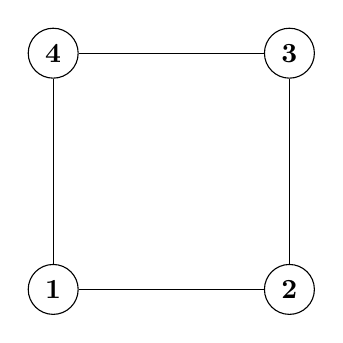
\begin{tikzpicture}
        \node (1)[draw , circle] at (0,0) {\textbf{1}};
        \node (2)[draw , circle] at (3,0) {\textbf{2}};
        \node (3)[draw , circle] at (3,3) {\textbf{3}};
        \node (4)[draw , circle] at (0,3) {\textbf{4}};
        
        \draw (1) -- (2);
        \draw (2) -- (3);
        \draw (3) -- (4);
        \draw (4) -- (1);
        
    \end{tikzpicture}    
\end{center}



\subsection{Task-2}
Draw a directed graph with nodes Home, School, Library and Park. Use arrows for these paths:
Home to School, School to Library, Library to Park, and Park to Home.\\


\begin{center}
    \begin{tikzpicture}
        \node (Home)[draw] at (0,0) {\textbf{Home}};
        \node (School)[draw] at (6,0) {\textbf{School}};
        \node (Library)[draw] at (6,-6) {\textbf{Library}};
        \node (Park)[draw] at (0,-6) {\textbf{Park}};

        \draw [->] (Home) -- (School);
        \draw [->] (School) -- (Library);
        \draw [->] (Library) -- (Park);
        \draw [->] (Park) -- (Home);
    \end{tikzpicture}
\end{center}


\subsection{Task-3}
Copy the graph from Task 2.2 and add a distance label (for example 2 km) on every edge. Place
the labels so they do not overlap the lines.\\


\begin{center}
    \begin{tikzpicture}
        \node (Home)[draw] at (0,0) {\textbf{Home}};
        \node (School)[draw] at (6,0) {\textbf{School}};
        \node (Library)[draw] at (6,-6) {\textbf{Library}};
        \node (Park)[draw] at (0,-6) {\textbf{Park}};

        \draw [->] (Home) -- node[above]{2km} (School);
        \draw [->] (School) -- node[right]{2km}(Library);
        \draw [->] (Library) -- node[below]{2km}(Park);
        \draw [->] (Park) -- node[left]{2km}(Home);
    \end{tikzpicture}
\end{center}

\newpage

\section{LEVEL-3:}
Shapes and Formatting
\subsection{Task-1}
Define a style named vertex (circle, colored fill, thick outline). Redraw your graph from Task 2.1
using this style on every node. Make the diagonal edge dashed and red.\\


\textbf{Shapes and Formatting}
\begin{center}
    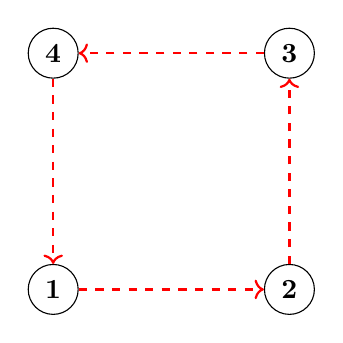
\begin{tikzpicture}
    \tikzset{
    vertex/.style={
        circle,
        colored-fill=red!20,
        
    }
    }
        \node (1)[draw , circle] at (0,0) {\textbf{1}};
        \node (2)[draw , circle] at (3,0) {\textbf{2}};
        \node (3)[draw , circle] at (3,3) {\textbf{3}};
        \node (4)[draw , circle] at (0,3) {\textbf{4}};
        
        \draw[-> ,thick,red, dashed] (1) -- (2);
        \draw[-> ,thick,red, dashed] (2) -- (3);
        \draw[-> ,thick,red, dashed] (3) -- (4);
        \draw[-> ,thick,red, dashed] (4) -- (1);
        
    \end{tikzpicture}    
\end{center}



\subsection{Task-2}
Define a second style named road for edges (thick, an arrow tip with Stealth, a color of your
choice). Redraw Task 2.2 using vertex for the nodes and road for every edge. Use at least two
different node colors (for example, one color for Home).\\


\begin{center}
    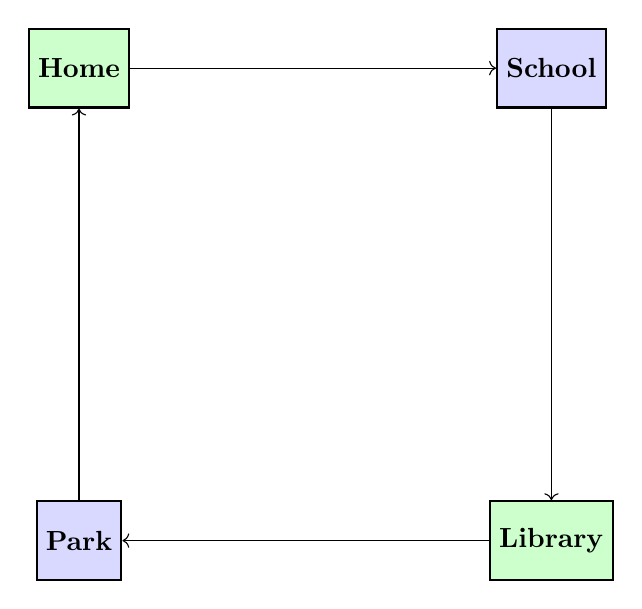
\begin{tikzpicture}
    \tikzset{
    vertex/.style={
        draw,
        thick,
        fill=blue!15,
        minimum size=1cm
    },
    road/.style={
        thick,
        ->,
        Stealth,
        brown
    }
}
         \node[vertex, fill=green!20] (Home) at (0,0) {\textbf{Home}};
         
        \node[vertex] (School) at (6,0) {\textbf{School}};
        
        \node[vertex, fill=green!20] (Library) at (6,-6) {\textbf{Library}};
        
        \node[vertex] (Park) at (0,-6) {\textbf{Park}};

        \draw [->] (Home) -- (School);
        \draw [->] (School) -- (Library);
        \draw [->] (Library) -- (Park);
        \draw [->] (Park) -- (Home);
    \end{tikzpicture}
\end{center}


\newpage
\section{LEVEL-4}
\textbf{Connecting Graphs}\\
\subsection{Task-1}
Draw a graph with five nodes A–E using only relative positions (right=of, below=of); do not use
at (x,y). Connect them in a chain A–B–C–D–E.\\


\begin{center}
    \begin{tikzpicture}[node distance=2cm]
        \tikzset{
            vertex/.style=
            {
                draw,
                circle,
                thick,
                fill=blue!15,
                minimum size = 1cm
            },
            road/.style=
            {
                dashed,
                fill=red!15,
                ->
            }
        }
    \node[vertex] (A) {\textbf{A}};
    \node[vertex, right=of A] (B) {\textbf{B}};
    \node[vertex, right=of B] (C) {\textbf{C}};
    \node[vertex, below=of C] (D) {\textbf{D}};
    \node[vertex, left=of D]  (E) {\textbf{E}};


    \draw[road] (A) -- (B);
    \draw[road] (B) -- (C);
    \draw[road] (C) -- (D);
    \draw[road] (D) -- (E);
    \draw[road] (B) -- (E)
    \draw[road] (E) -- (A);
    \end{tikzpicture}
\end{center}

\subsection{Task-2}
Draw two nodes X and Y joined by two curved arrows (one each way). Add a loop on X and a
loop on Y.\\


\begin{center}
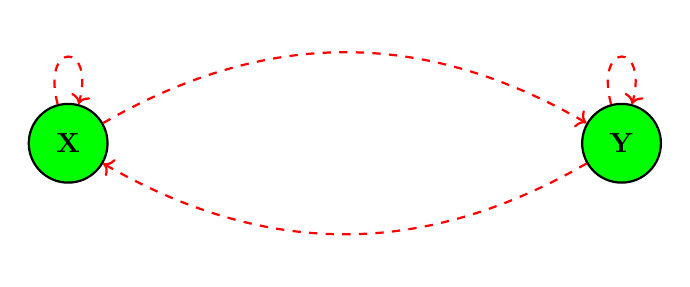
\begin{tikzpicture}[node distance = 6 cm]
    \tikzset{
    vertex/.style=
    {
        circle,
        draw,
        thick,
        fill=green!100,
        minimum size = 1cm
    },
    road/.style=
    {
        thick,
        dashed,
        red,
        ->
    }
}

  \node[vertex] (X) {\textbf{X}};
  \node[vertex, right =of X] (Y) {\textbf{Y}};

  \draw[road, bend left] (X) to (Y);
  \draw[road, bend left] (Y) to (X);
  \draw[road] (X) to [loop above] (X);
  \draw[road] (Y) to [loop above] (Y);

\end{tikzpicture}
\end{center}
\newpage

\subsection{Task-3}
Draw two small graphs of your own (at least three nodes each) and connect them with a dashed
bridge edge. Use the vertex style from Level 3.\\


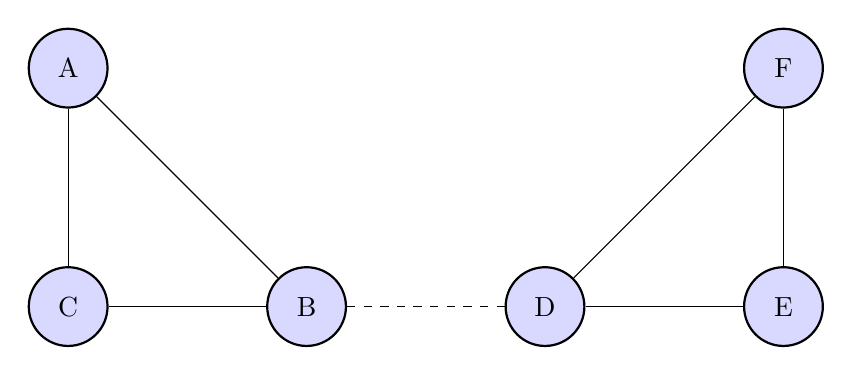
\begin{tikzpicture}[node distance=2cm]

    \tikzset{
        vertex/.style={
            draw,
            circle,
            thick,
            fill=blue!15,
            minimum size=1cm
        }
    }
    \node[vertex] (A) {A};
    \node[vertex, below=of A] (C) {C};
    \node[vertex, right=of C] (B) {B};

    \draw (A) -- (B);
    \draw (A) -- (C);
    \draw (B) -- (C);

    \node[vertex, right= of B] (D) {D};
    \node[vertex, right=of D] (E) {E};
    \node[vertex, above=of E] (F) {F};

    \draw (D) -- (E);
    \draw (D) -- (F);
    \draw (E) -- (F);

    \draw[dashed] (B) -- (D);

\end{tikzpicture}
\end{document}
